%XeLaTeX+makeIndex+BibTeX OR LuaLaTeX+...
\documentclass[a4paper,12pt]{article} %14pt - extarticle
\usepackage[utf8]{inputenc} %русский язык, не менять
\usepackage[T2A, T1]{fontenc} %русский язык, не менять
\usepackage[english, russian]{babel} %русский язык, не менять
\usepackage{fontspec} %различные шрифты
\setmainfont{Times New Roman}

%\defaultfontfeatures{Ligatures={TeX},Renderer=Basic}
\usepackage[hyphens]{url} %ссылки \url с переносами
\usepackage{hyperref} %гиперссылки href
\hypersetup{pdfstartview=FitH,  linkcolor=blue, urlcolor=blue, colorlinks=true} %гиперссылки
\usepackage{subfiles}%включение тех-текста
\usepackage{graphicx} %изображения
\usepackage{float}%картинки где угодно
\usepackage{textcomp}


%\usepackage[dvips]{color} %попытка добавить цвета типа OliveGreen. Пропадают все картинки

\usepackage{dsfont}%мат. символы
%\usepackage[style=gost-footnote]{biblatex} %ГОСТ https://www.ctan.org/pkg/biblatex-gost С ним только хуже! Не использовать его!
\newcommand{\ovr}[1]{\overrightarrow{#1}}
\usepackage{listings} %code formatting
\lstset{language=sql,keywordstyle=\color{blue},tabsize=2,breaklines=true,
morekeywords={if, CONCAT, is}}
%хорошая статья об этом пакете: http://mydebianblog.blogspot.com/2012/12/latex.html

\addto\captionsrussian{\def\refname{Использованные источники}}

\begin{document}
\title{Описание проекта <<Тренажёр Брайля>>}
\author{Валерий Зуев}
\maketitle
\section{Краткое описание}
Предлагается собрать и запрограммировать \textbf{тренажёр Брайля} -- прибор для обучения слепых людей \textbf{шрифту Брайля}. Идея шрифта Брайля -- представление буквы в виде группы выпуклых точек, оттиснутых на бумаге или иной поверхности (иногда такие есть на упаковках с лекарствами). Слепые могут читать на ощупь, но должны выучить обозначение каждой буквы.\\
Основной элемент прибора -- электромеханическая \textbf{ячейка Брайля}, которая посредством сервоприводов воспроизводит буквы шеститочечного шрифта Брайля. Планируется, ориентируясь на разработанный заблаговременно прототип ячейки, создать несколько обучающих программ для ПК или одноплатного компьютера Nano Pi. Непосредственно управлять сервоприводами будет контроллер Arduino Uno; планируется написать программу для него. Помимо того, планируется усовершенствовать и доработать ячейку Брайля.

\section{Актуальность}
Число инвалидов по зрению в России по состоянию на 2011 год оценивалось в 103 тысячи человек, и предполагается дальнейшее увеличение их количества\cite{stat}. При этом число людей, владеющих шрифтом Брайля, снижается \cite{brailleLower}. Причина как в относительной дороговизне специальных книг, так и в сложности обучения, в неразвитости системы обучения. При этом знание шрифта Брайля позволяет слепому читать, учиться и даже работать.\\
В настоящее время выпускаются дисплеи Брайля -- приставки к компьютеру с компактными пьезоэлектрическими ячейками. Эти устройства позволяют читать до 80 символов Брайля одновременно и вводить текст с помощью особой клавиатуры из восьми клавиш (по одной на каждую точку в букве азбуки Брайля). Основной их недостаток -- цена (в среднем 150 тысяч русских рублей по состоянию на январь 2019 года).

\section{Предшествующие работы}
Были предприняты многочисленные попытки создания более доступного дисплея Брайля.  В их числе нитиноловые \cite{sma}, на основе электрической стимуляции кожи \cite{kaji1} \cite{kaji2}, на основе электромоторов \cite{bristol}, круговые \cite{rotDisp}. В 2016 году автор статьи пытался разработать собственную конструкцию кругового дисплея Брайля (рис. \ref{myRoundDisp}), но из-за сложности создания миниатюрной механики проект был свёрнут.\\

\begin{figure}[h!]
\center{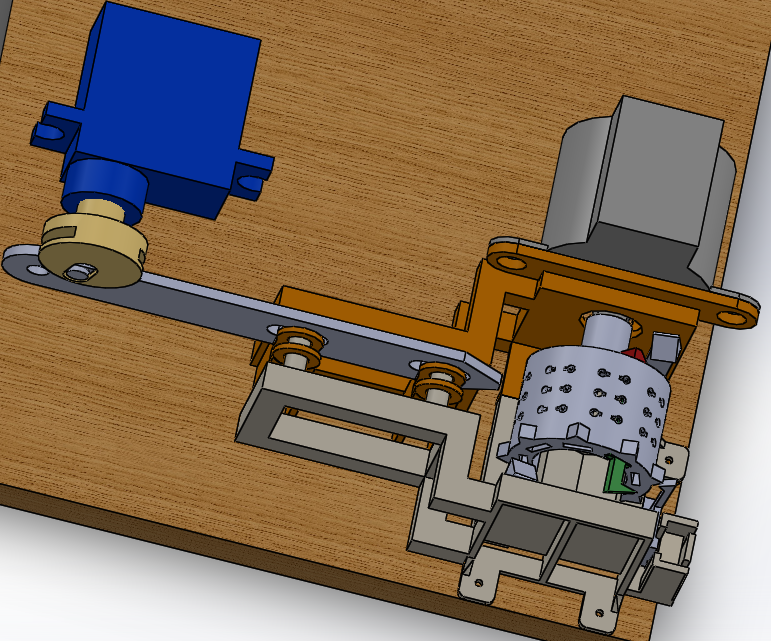
\includegraphics[width=.75\textwidth]{pictures/screen5.png}}
\caption{Компьютерная модель нереализованного кругового дисплея Брайля}
\label{myRoundDisp}
\end{figure}

В 2016-2017 годах команда под руководством магистра кафедры <<Теоретическая Механика>> Глеба Андреевича Мирошника создала несколько прототипов тренажёра Брайля - дисплея с одной ячейкой, ориентированного на обучение слепых, а не на длительное чтение \cite{gleb}. После ряда попыток создать ячейку Брайля на основе сервоприводов было решено отказаться от них в пользу обычной, более надёжной пьезоэлектрической ячейки. Такой тренажёр компактный, но трудновоспроизводимый: ячейки дисплея Брайля, по имеющимся данным, не продаются отдельно от дисплеев.

\section{Цели работы}
Цель - создать надёжный и простой в изготовлении тренажёр Брайля и комплекс программ для него. Предлагается развить идею, реализованной командой Г. А. Мирошника. Ячейка Брайля будет создана с применением только доступных компонентов (сервоприводов, контроллеров Arduino и/или Raspberry Pi, деталей, пригодных к изготовлению на большинстве 3D-принтеров). За счёт открытого распространения материалов проекта предполагается возможным легко воспроизводить дисплей и сделать обучение шрифту Брайля доступным для людей по всему миру.

\section{Описание конструкции}
Создан прототип ячейки (рис. \ref{photo1}). Точки символа Брайля - головки подвижных штырьков. Штырьки приклеены к рычагам и двигаются вверх-вниз, отчего точки появляются над поверхностью или убираются внутрь. Движение обеспечивают сервоприводы с насаженными на вал шестернями. Каждый рычаг на противоположном от штырька конце имеет зубчатую рейку, которой передаётся движение шестерни.

\begin{figure}[h!]
\center{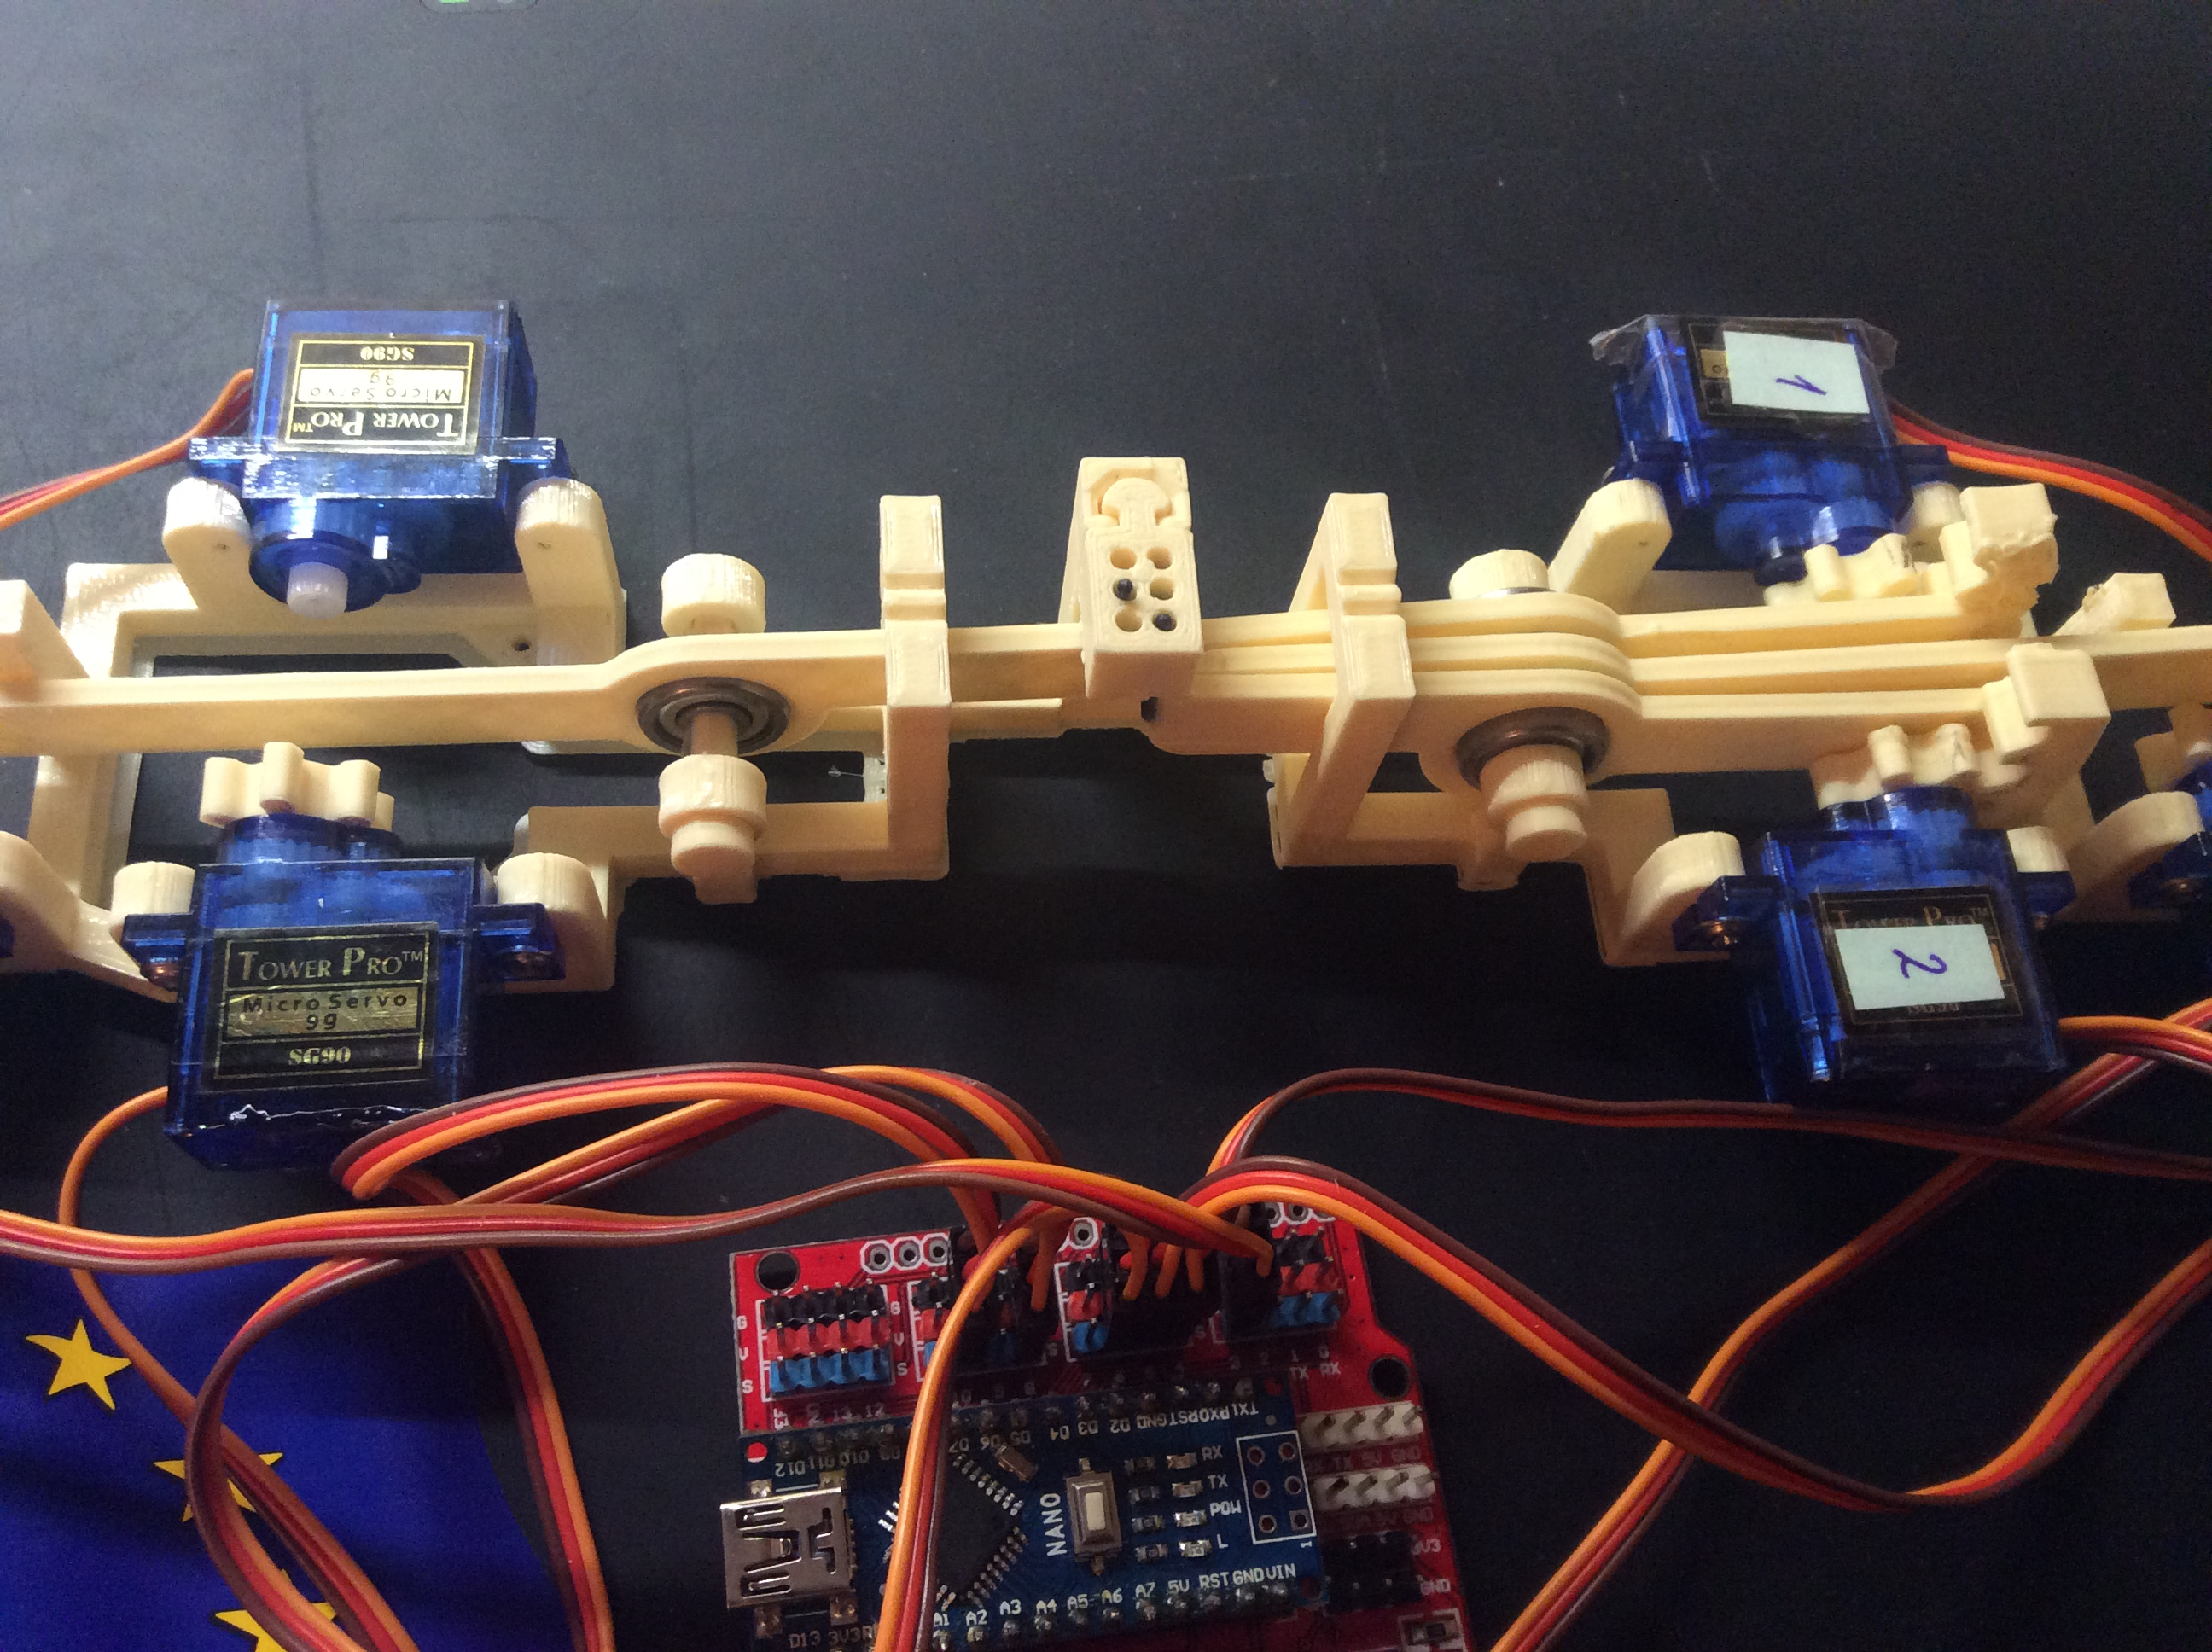
\includegraphics[width=.75\textwidth]{pictures/photo1.jpg}}
\caption{Прототип ячейки Брайля}
\label{photo1}
\end{figure}

\section{Текущие задачи и планируемое решение задач}
\subsection{Базовые задачи}
\begin{itemize}
\item{}Написать программу для Arduino, которая выводит текст, отправленный через Serial.
\item{}Снабдить дисплей органами управления (кнопки или джойстик). По нажатию кнопки передавать сигнал по Serial.
\item{}Составить два обучающих приложения на Python, общающихся с Arduino через Serial. Одно для запоминания азбуки: воспроизводит на экране буквы и сопровождает звуком; второе - тест на знание азбуки: дисплей выводит букву, пользователь должен произнести её вслух. Компьютер определяет с помощью распознавания голоса, верно ли ответил пользователь.
\item{}Спроектировать и создать корпус устройства
\item{}Разместить материалы проекта в свободном доступе (к примеру, на платформе Github), чтобы предоставить возможность создания подобного прибора всем желающим.
\end{itemize}
\subsection{Приблизительный список дополнительных задач}
\begin{itemize}
\item{}Адаптировать программы на Python к контроллеру Raspberry Pi/Nano Pi. Создать отдельный опциональный модуль хост-контроллера с динамиком и микрофоном в собственном корпусе.
\item{}Составить меню тренажёра Брайля (список приложений) с возможностью навигации джойстиком. Названия пунктов меню выводятся с помощью ячейки Брайля или произносятся вслух динамиками компьютера.
\item{}Написать иные программы (обучающие или, возможно, для чтения текста). Пример - часы (показать время с помощью ячейки Брайля).
\item{}Повысить компактность ячейки Брайля: взять подшипники меньшего размера, перекомпоновать сервоприводы (разместить два из них на другой стороне рычагов).
\item{}Попробовать управлять серво с помощью ШИМ контроллера PCA9685
\item{}Создать ячейку с восемью точками (расширенный шрифт Брайля).
\item{}Снабдить тренажёр особой клавиатурой из восьми клавиш. Снабдить встроенным динамиком и, возможно, лампочками для зрячего иструктора (индикатор питания и подключения хост-контроллера).
\item{}Предусмотреть в конструкции механизм для автокалибровки ячейки.
\item{}Уделить внимание не техническим аспектам (презентовать проект, возможно, создать видеоклип/сайт проекта).
\end{itemize}


\begin{thebibliography}{99}
\bibitem{gleb}{Тренажёр Брайля. Глеб Андреевич Мирошник. [Электронный ресурс] \url{http://www.brailletrainer.ru}}
\bibitem{sma}{Microtuators of SMA for Braille display system \url{https://www.researchgate.net/publication/232633029_Microtuators_of_SMA_for_Braille_display_system}}
\bibitem{kaji1}{Electro-Tactile Display with Force Feedback. Hiroyuki Kajimoto, Naoki Kawakami, Taro Maeda and Susumu Tachi: Graduate School of Information Science and Technology, The University of Tokyo. [Электронный ресурс]. \url{http://citeseerx.ist.psu.edu/viewdoc/download?doi=10.1.1.493.2786&rep=rep1&type=pdf}}
\bibitem{kaji2}{Electro-Tactile Display with Tactile Primary Color Approach.
Hiroyuki Kajimoto, Naoki Kawakami, Susumu Tachi. Graduate School of
Information Science and Technology, The University of Tokyo.  [Электронный ресурс]. \url{http://files.tachilab.org/publications/intconf2000/kajimoto200410IROS.pdf}}
\bibitem{bristol}{Bristol Braille technology [Электронный ресурс] \url{http://bristolbraille.co.uk}}
\bibitem{rotDisp}{Refreshable braille reader. John W. Roberts, Oliver T. Slattery, David W. Kardos. [Электронный ресурс] \url{https://patents.google.com/patent/US6776619}}
\bibitem{stat}{Оценка динамики и прогноз первичной инвалидности в Амурской области вследствие офтальмопатологии. Выдров А. С. [Электронный ресурс] \url{https://cyberleninka.ru/article/v/otsenka-dinamiki-i-prognoz-pervichnoy-invalidnosti-v-amurskoy-oblasti-vsledstvie-oftalmopatologii}}
\bibitem{brailleLower}{Актуальность рельефно-точечного шрифта по системе брайля в современном мире. [Электронный ресурс] \url{https://beltiz.by/talking/1068-2013-12-19-11-49-03}}
\bibitem{blindLib1}{М. П. Коновалова,  О. Ю. Жарова. Технические средства реабилитации для людей с ограниченными возможностями (на примере опыта работы Калужской областной специальной библиотеки для слепых им. Н. Островского) (окончание). [Электронный ресурс] \url{https://cyberleninka.ru/article/v/tehnicheskie-sredstva-reabilitatsii-dlya-lyudey-s-ogranichennymi-vozmozhnostyami-na-primere-opyta-raboty-kaluzhskoy-oblastnoy-1}}
\end{thebibliography}
\end{document}